\section{Embedded Systems}
Keywords: Mikroprozessortechnik, Mikroprozessor, Mikroarchitektur

\begin{itemize}[nosep]
	\item Echtzeitfühigkeit
	\item Zuverlässigkeit
	\item Informationssicherheit
	\item Ressourcen	
	\item Kostendruck	
\end{itemize}
~\\
DSP: in audio, video, AI etc
\\
SoC: ASIC, FPGA, Soft-Core

\subsection{Bestandteile}
\begin{itemize}[nosep]
	\item CPU
	\item Speicher (RAM, ROM)
	\item I/O Einheiten
	\item Systembus $\rightarrow$ Master-Slave-Prinzip
	\item IRQ Fähigkeit
	\item Timer, OZI
\end{itemize}

\subsubsection{Architektur}
\subsection{Architektur}
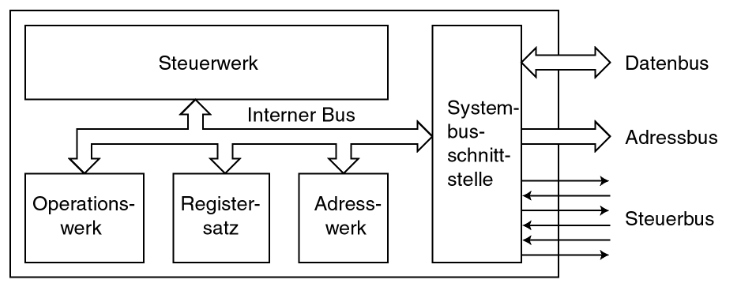
\includegraphics[width=\columnwidth]{Images/Blockschema}
Der \textbf{Registersatz} enthält einen Satz von Registern,  mit dem Daten innerhalb des Prozessors  gespeichert  werden  können.   Ein  Register  ist  eine  Gruppe  vonFlipflops mit gemeinsamer Steuerung.\\
Das \textbf{Operationswerkführt}  die  eigentliche  Verarbeitung,  d.h.   die  logischen  und arithmetischen Operationen, an den übergebenen Daten aus.\\
Das \textbf{Steuerwerk ist} verantwortlich für die Ablaufsteuerung sowohl im Inneren des Prozessors als auch im restlichen System.\\
Das \textbf{Adresswerk} erzeugt die erforderlichen Adressen, um auf Daten und Code im Hauptspeicher zugreifen zu können.\\
Die \textbf{Systembus-Schnittstelle} enthält Puffer- und Treiberschaltungen, um den Datenverkehr über den Systembus abzuwickeln.

~\\
\begin{itemize}[nosep]
	\item Neumann vs Havard
		\begin{itemize}[nosep]
			\item Von-Neumann $\rightarrow$ Gleicher Systembus, Bottleneck!
			\item Havard $\rightarrow$ ein Bus für Daten, einer für Programm!
		\end{itemize}
	\item Mikroprozessor vs Mikrocontroller (RAM)
\end{itemize}

\begin{itemize}[nosep]
	\item CISC vs RISC
	\begin{itemize}[nosep]
		\item CISC besitzen viele spezialisierte Instruktionen.
		\item RISC besitzen wenige dafür einfache Instruktionen.
	\end{itemize}
\end{itemize}

\subsection{Polling/IRQ}
\todo{Woche 03}